\chapter{Introduction}
\lhead{\emph{Introduction}}
\label{chapter:intro}

 Whether it be within a virtual space such as in a video game or training simulation \cite{alexander2005gaming}, or within a remote real world location as in telerobotics, a feeling of presence \cite{presence} allows the user to more naturally and intuitively interact with the presented environment as if they were truly there. The desire for presence within a space that is not your own is therefore one that drives much technological innovation. In telerobotics in particular, where the aim can often be to interact with dangerous or industrial environments, intuitive control is essential to safe and effective operation.

Virtual Reality (VR) is a technology spearheaded by the video games industry for use in immersive gaming applications. Through the use of a tracked headset, giving the user the ability to freely look around a 3D space, it provide unparalleled presence within a virtual world---comparable to presence within a real, physical space \cite{loomis2016presence,McGlynn}. To be able to incorporate VR into teleoperation is therefore desirable, however, sending a video feed to the headset as if it were a normal monitor has been found to lead to motion sickness \cite{han2017design}. This is due to VR's high frame rate and low latency requirements. It's widely accepted that for a VR application to not cause motion sickness and headaches due to frame rate, it must maintain at least 90 frames per second (fps) \cite{FrameRate}; a minimum of 60 fps can also be acceptable \cite{Borg2013UsingAG}, but generally only for applications with little motion or when used by people with lower susceptibility to motion sickness. Unfortunately, to transmit 90 fps from a stereo camera rig (two images are required to perceive 3D) to the computer running the VR application has bandwidth requirements too high to be currently implementable outside the most expensive of designs.

Another consideration is the ability to look around the space independently, as this is a major factor in providing presence to the user in VR. This can be achieved by mounting the stereo camera rig on a gimbal, however to build a gimbal that is able to track the angle of the user's head accurately and with low latency is, once again, expensive and challenging \cite{DORA}; if not implemented perfectly the user would experience significant sickness and dissociation from the space.

The aim of this project is to research the use of data abstraction to minimise the outlined technical issues through the design and implementation of a telerobotics system that incorporates it. To achieve this, the system must reduce each image down to its most essential features, reducing its size and therefore the required bandwidth significantly. Each image pair must then be transmitted to a server and combined into a single 3D model of the space that could be looked around freely through the VR headset. As the camera feed is converted to a 3D model rather than displayed directly as images, the headset could run at its maximum frame rate of 90 fps even if the model is updating at a much slower rate. The use of abstraction has the capacity to allow for high presence systems, as presence in VR is not dependant on the 3D environment being an exact reproduction of the telerobot's space, only that the reproduction is consistent and comfortable to view. 

\begin{figure}[H]
    \begin{center}
      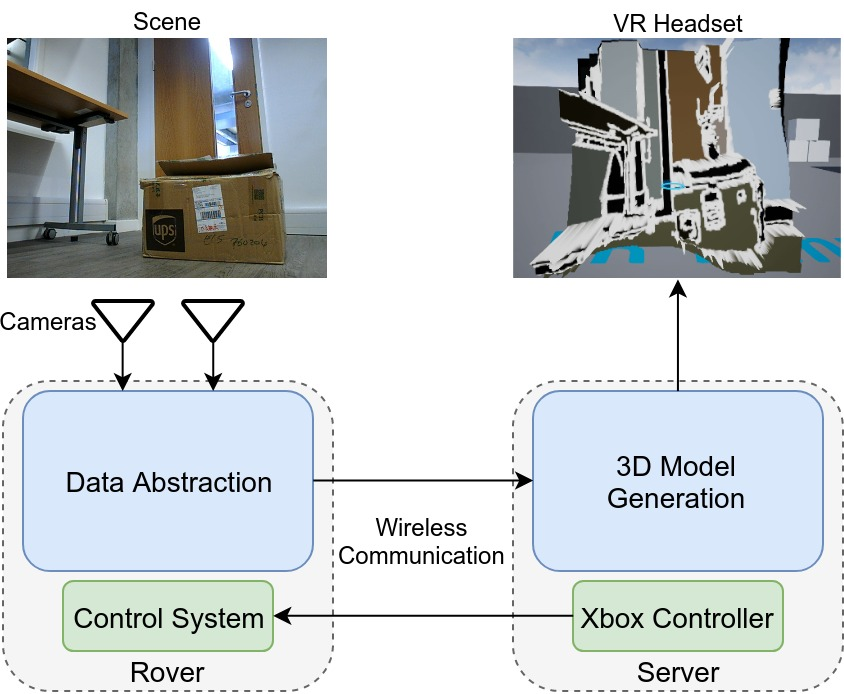
\includegraphics[width=0.7\textwidth]{Figures/Outline.jpg}
      \caption[System Outline]{System Outline. It can be seen that the scene the rover's cameras are observing (top left) is within the VR environment (top right) as a simple abstracted 3D representation.}
      \label{fig:outline}
    \end{center}
\end{figure}

The system (cf. Figure \ref{fig:outline}) consists of two platforms: a server (Chapter \ref{chapter:server}) that runs a VR environment and reads user input from an Xbox 360 controller, and a rover platform (Chapter \ref{chapter:rover}) that is controlled from said environment and supplies the abstracted images that the 3D model in the environment is built from. The rover (Figure \ref{fig:marvin}) is a simple drivable platform with a stereo camera gimbal mounted on it (adapted from one produced by previous students \cite{gimble}). The server is a powerful PC running Windows 10 \cite{windows} and a HTC Vive \cite{Vive}. The data abstraction algorithm the system uses is novel, so its design and development is initially discussed in isolation (Chapter \ref{chapter:abstract}), and then its implementation within the system explained as part of the rover implementation (Chapter \ref{chapter:rover}).

\begin{figure}[H]
    \begin{center}
      \begin{tabular}{ c }
        \includegraphics[width=0.65\textwidth]{Figures/marvin.jpg} \\
        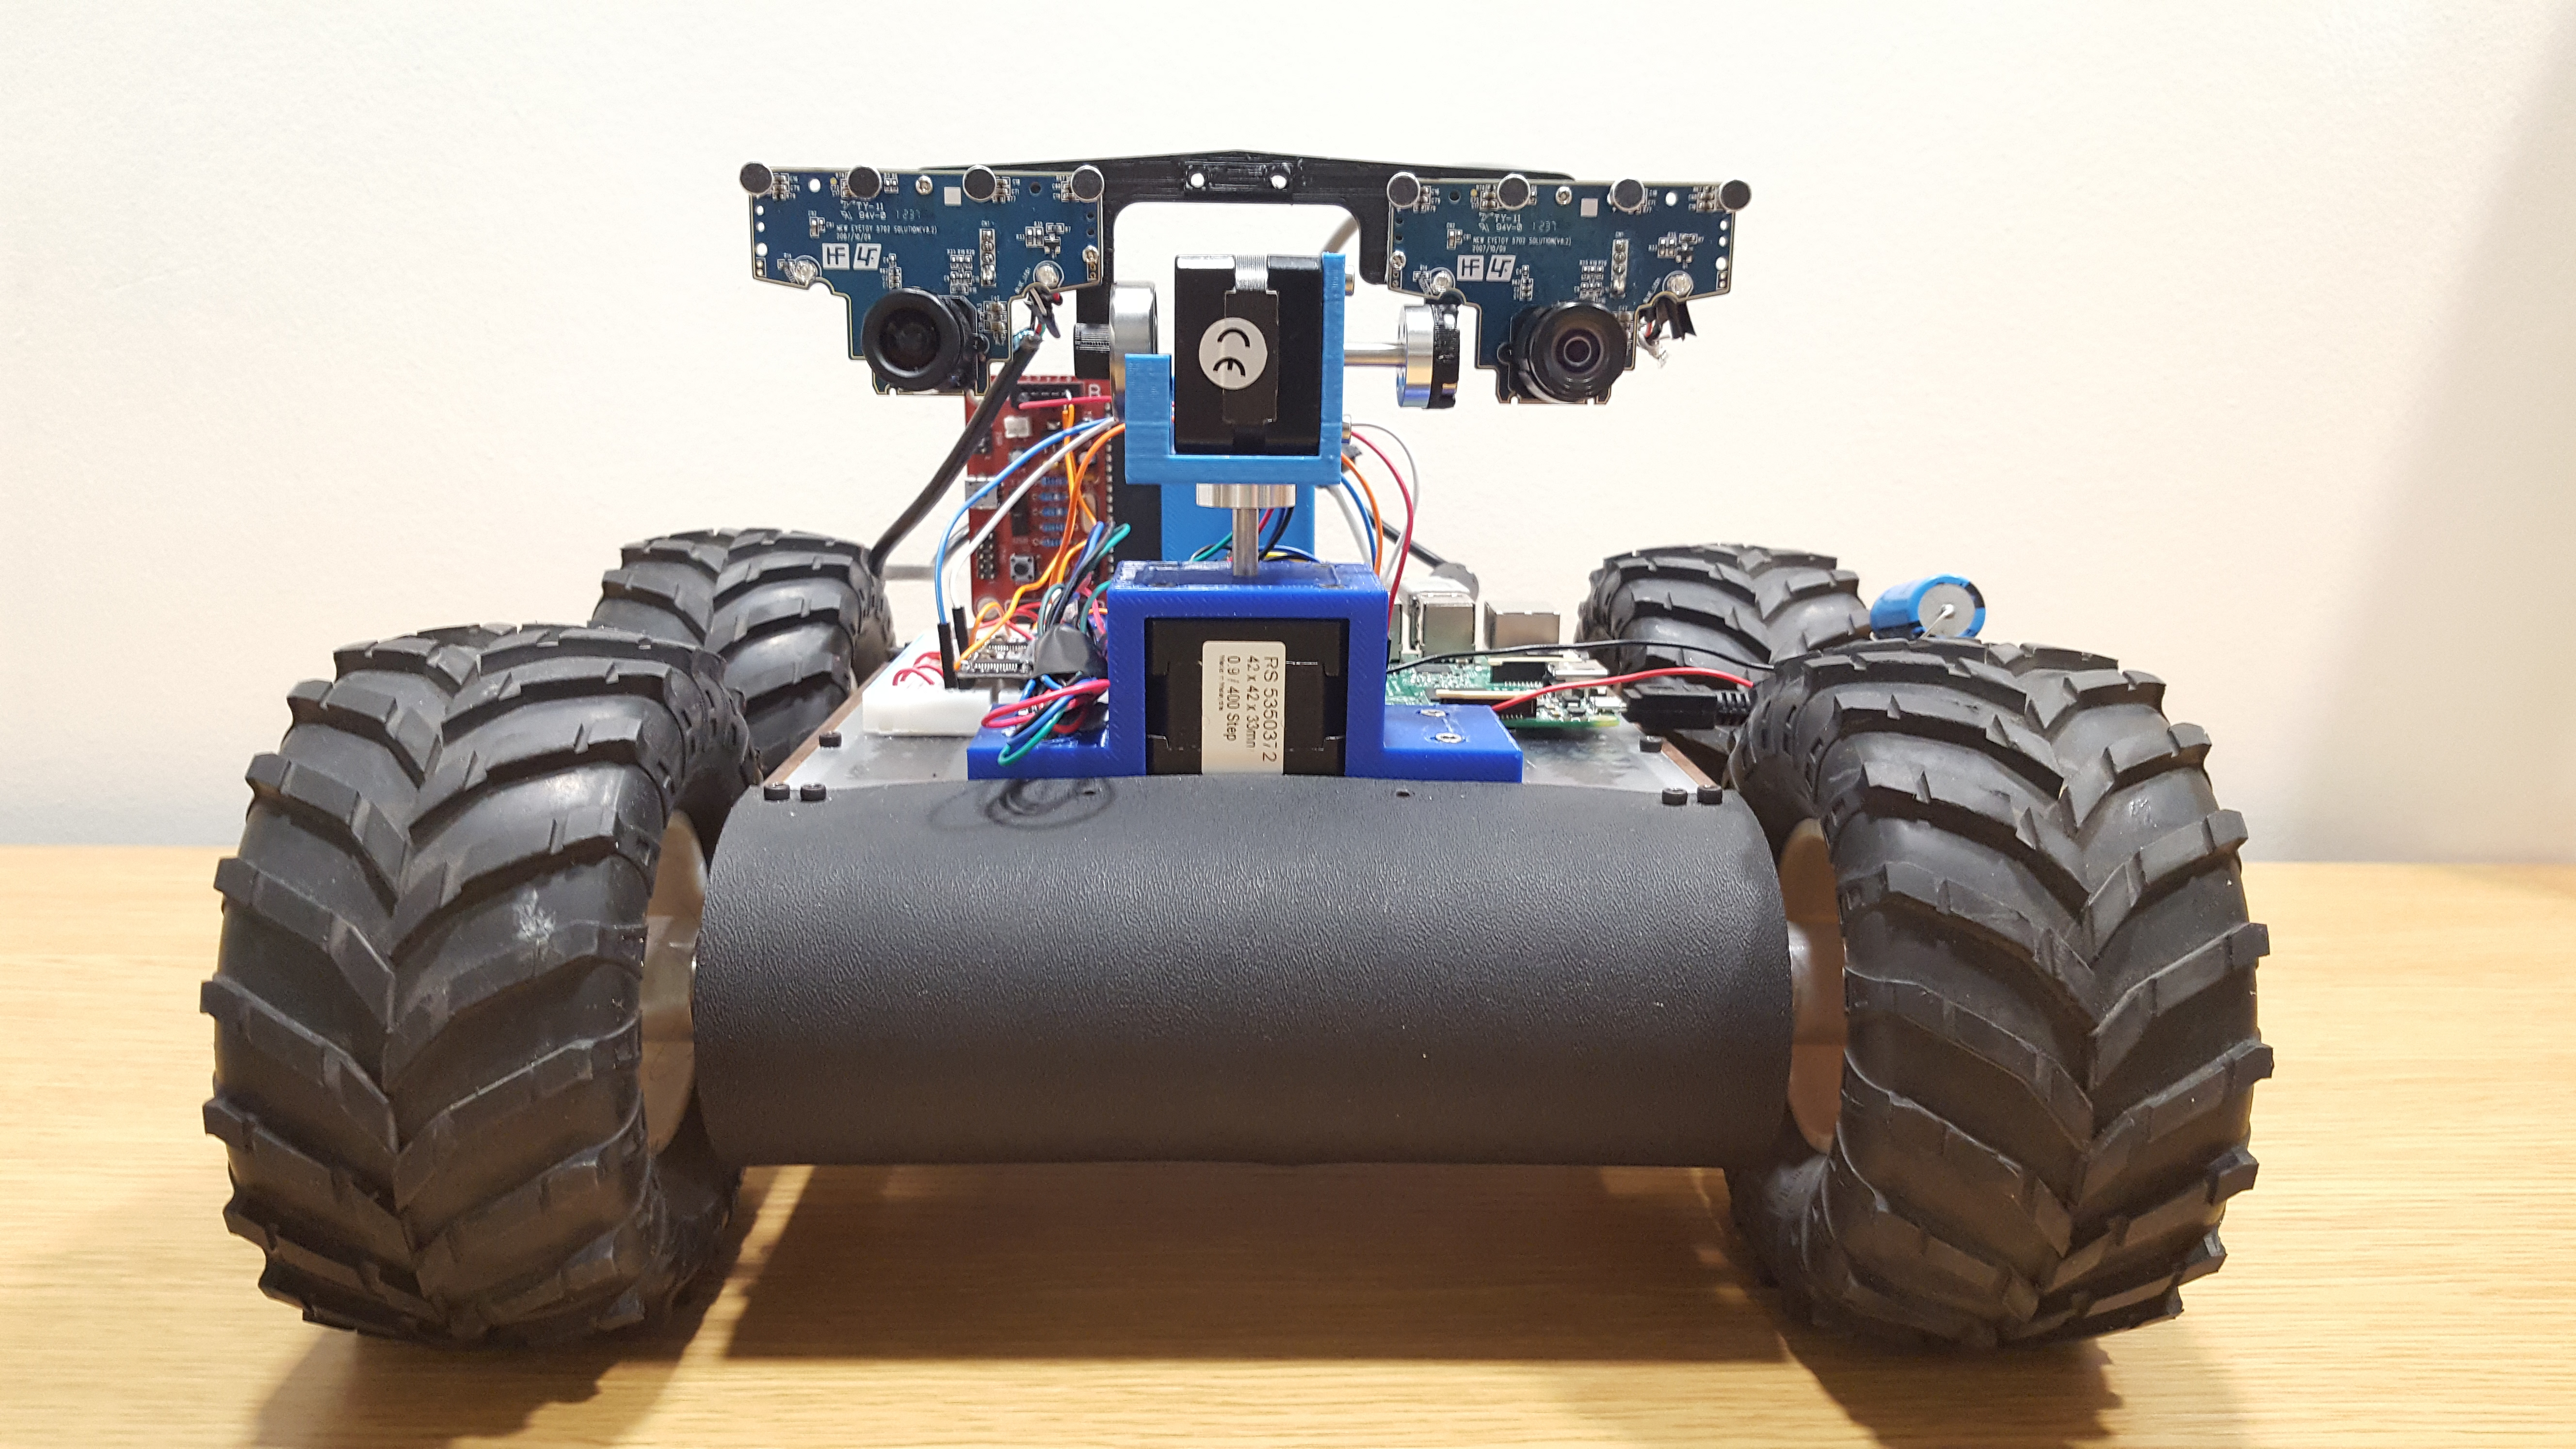
\includegraphics[width=0.65\textwidth]{Figures/marvinF.jpg} \\
        \includegraphics[width=0.65\textwidth]{Figures/marvinS.jpg} \\
        \includegraphics[width=0.65\textwidth]{Figures/marvinT.jpg}
      \end{tabular}
      \caption[Rover Pictures]{Rover Pictures.}
      \label{fig:marvin}
    \end{center}
\end{figure}